\chapter{Introduction to P/Invoke}

\section{Getting Started}
First, create a Directory as 'ChapterTwo' for this project and create a new file, 'ChapTwo.c' under 'ChapterTwo' folder.

Let's assume we have a basic Addition function in a C Library that we want to call.

\begin{lstlisting}{c}
int Sum(int a, int b)
{
  return a+b;
}
\end{lstlisting}

It's a simple Addition Operation at a first glance, but there are\newline considerations that must be observed first before attempting to write platform invocation wrapper code for the function above:

\begin{enumerate}
	\item \label{itm:first} `int` datatype in C can be considered 2 bytes long or 4 bytes long or however long it may be depending on the architecture and compiler that the library is compiled on. In C Standard, int must be capable of containing \textbf{at least} the [\textminus32,767, +32,767] range; thus, it is at least 16 bits in size.
	
	\item Due to \ref{itm:first}, you can reasonably safeguard against data loss by substituting C\# Int32(int) which contains 4 bytes or you may choose follow the standard strictly by supplying C\# Int16(short) which contains 2 bytes, even though it can suffer data loss. The best approach is to avoid using "at least" integers in C and instead use fixed size integers provided by the compiler in ''stdint.h'' header if you have Foreign Function Interface kept in mind.
	
	\item Sometimes you have to keep Endianess in mind although it is less of a concern in x86\_64 architecture since little endianess is the default.
\end{enumerate}
\newpage
The best approach to writing the Addition function is to make it clear what sized integers you're attempting to add  if possible.

\begin{lstlisting}{c}
#include <stdint.h>
int32_t Sum(int32_t a, int32_t b)
{
  return a+b;
}
\end{lstlisting}

\section{Compiling the Library}
This book assumes you have sufficient knowledge of C, we will still however, provide compilation instruction. The following command assumes that you have named your source code file as 'ChapTwo.c' as instructed at the beginning of this chapter.

\begin{lstlisting}
clang -std=c99 -shared -fPIC -olibChapTwo.so ChapTwo.c
\end{lstlisting}

Here we examine and explain the compiler arguments:

\begin{enumerate}
	\item '-std=c99' specify that we are compiling C source code under C99 Standard.
	\item '-shared' specify that we want the program to be compiled as shared/dynamic library.
	\item '-fPIC' specify that code must be position independent so that the resultant library can be loaded by other processes and have code be made available to be run anywhere in program address space regardless of code's address.
	\item '-olibChapTwo.so' specify what the output library should be named. lib prefix in 'libChapTwo.so' is a matter of naming convention to be followed on Linux although compilers like clang and gcc do search libraries based on lib prefix when using '-l' option. 
\end{enumerate}
\newpage
\section{Configuring C\# Project}
Since we're already in "ChapterTwo" directory, we can go ahead and run 'dotnet new Console'. There are a few steps we need to take to add the C code to our C\# project. First, we need to automate the compilation process of our C file and copy the compiled C library to the target directory for Debug, Release, or any other configurations.

Open up 'ChapterTwo.csproj' file with your favorite editor, and add the following under '</PropertyGroup>' inside '<Project>' tag.

\begin{lstlisting}{language=XML}
<Target Name="CompileCProject" AfterTargets="AfterBuild">
	<exec Command=
	"clang -std=c99 -shared -fPIC -olibChapTwo.so
	ChapTwo.c" />
	<Copy SourceFiles="libChapTwo.so" DestinationFolder="$(OutDir)" />
</Target>
\end{lstlisting}

The snippet above does few things after building our C\# project:
\begin{enumerate}
	\item Compile ChapTwo.c code as a shared library, libChapTwo.so
	\item Copy libChapTwo.so into any target directory that C\# is being built in.
\end{enumerate}

This makes it significantly easier to modify our code without having to run any additional commands for it to take effect.

Your CSProj should look like the following:

\begin{lstlisting}{language=XML}
<Project Sdk="Microsoft.NET.Sdk">

 <PropertyGroup>
  <OutputType>Exe</OutputType>
  <TargetFramework>netcoreapp2.0</TargetFramework>
 </PropertyGroup>
 <Target Name="CompileCProject" AfterTargets="AfterBuild">
  <exec Command="clang -std=c99 -shared -fPIC -olibChapTwo.so
ChapTwo.c" />
  <Copy SourceFiles="libChapTwo.so" DestinationFolder="$(OutDir)" />
 </Target>
</Project>
\end{lstlisting}
\newpage
\section{Wrapping C Code in C\#}
Open up Program.cs, add a new using directive at the top of your source code.

\begin{lstlisting}{c}
using System.Runtime.InteropServices;
\end{lstlisting}

This line imports all of the platform invocation services which enables us to interact with our C library with ease.

Add the following lines under Program class:

\begin{lstlisting}{c}
[DllImport("ChapTwo")]
static extern int Add(int a, int b);
\end{lstlisting}

The DllImport attribute declares that a static externally defined function is defined in a C library and to have CLR create a Platform Invocation stub to define the said function within external library.

It is required to declare the function with static and extern modifiers since it is a function that is both independent of state and externally defined.

Finally, modify the ''Console.WriteLine'' line to the following:

\begin{lstlisting}{c}
Console.WriteLine("1 + 2 = {0}", Add(1, 2)};
\end{lstlisting}
And your source code should look as follows:

\begin{lstlisting}{c}
using System;
using System.Runtime.InteropServices;
namespace ChapterTwo
{
	class Program
	{
		[DllImport("ChapTwo")]
		static extern int Add(int a, int b);
		static void Main(string[] args)
		{
		Console.WriteLine("1 + 2 = {0}", Add(1, 2));
		}
	}
}
\end{lstlisting}
\newpage
Finally, your program is ready to be executed. You can run:

''dotnet restore \&\& dotnet run''

And we have the following:

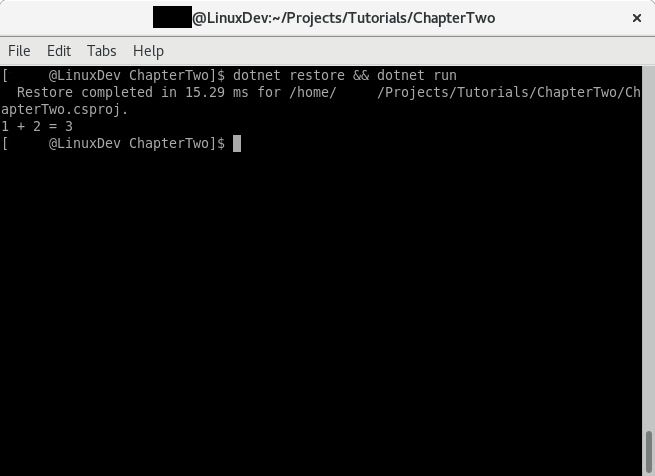
\includegraphics[width=\textwidth]{ChapTwoConsole}
It works as expected!
\newpage
\section{Some background}
There are few things happening when a function with DllImport is called, if this is the first time the function is being called, the Runtime will first load the external library immediately, then load the symbol ''Add'' by default, and finally generate a P/Invoke stub for that function to support the call to the external function.

The symbol is merely just that, a symbol that is exported by C Library. You can find a list of symbols by running ''objdump -T libChapTwo.so'' on your library and you'll have the following:

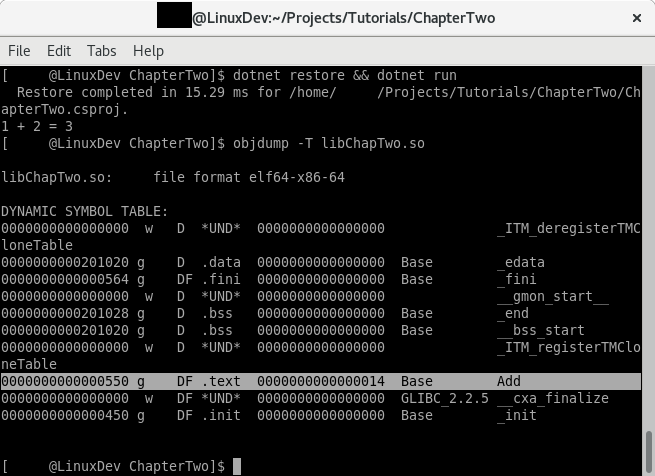
\includegraphics[width=\textwidth]{ChapTwoConsoleTwo}

You will notice that the Add symbol is shown in the symbol table in your library, this is how the CLR looks up a function by entry name.